%% LyX 2.4.0~beta5 created this file.  For more info, see https://www.lyx.org/.
%% Do not edit unless you really know what you are doing.
\documentclass[english]{foils}
\usepackage[T1]{fontenc}
\usepackage[latin9]{inputenc}
\pagestyle{foilheadings}
\setcounter{secnumdepth}{1}
\setcounter{tocdepth}{1}
\usepackage{color}
\usepackage{pifont}
\usepackage{amsmath}
\usepackage{amsthm}
\usepackage{amssymb}
\usepackage{graphicx}

\makeatletter
%%%%%%%%%%%%%%%%%%%%%%%%%%%%%% Textclass specific LaTeX commands.
\theoremstyle{remark}
\newtheorem*{rem*}{\protect\remarkname}
\theoremstyle{definition}
\newtheorem*{example*}{\protect\examplename}
\newenvironment{lyxcode}
	{\par\begin{list}{}{
		\setlength{\rightmargin}{\leftmargin}
		\setlength{\listparindent}{0pt}% needed for AMS classes
		\raggedright
		\setlength{\itemsep}{0pt}
		\setlength{\parsep}{0pt}
		\normalfont\ttfamily}%
	 \item[]}
	{\end{list}}
\theoremstyle{definition}
\newtheorem{defn}{\protect\definitionname}

%%%%%%%%%%%%%%%%%%%%%%%%%%%%%% User specified LaTeX commands.
\usepackage{xcolor}
\renewcommand{\labelitemi}{$\textcolor{blue}{\bullet}$}
\renewcommand{\labelitemii}{$\textcolor{teal}{\Rightarrow}$}
\renewcommand{\labelitemiii}{$\textcolor{red}{\rightarrow}$}
\renewcommand{\labelitemiv}{$\textcolor{brown}{\circ}$}
% for French theorems, etc. since I'm using English to fix bullet pb.
\providecommand{\examplename}{Example}
\providecommand{\definitionname}{Definition}
\providecommand{\theoremnname}{Theorem}
\providecommand{\remarkname}{Remark}
\providecommand{\exercisename}{Exercise}

\makeatother

\usepackage{babel}
\providecommand{\definitionname}{Definition}
\providecommand{\examplename}{Example}
\providecommand{\remarkname}{Remark}

\begin{document}

\MyLogo{Intro to ML}
\title{Supervised Learning - k-NN}
\author{Mark Asch - IMU/VLP/CSU }
\date{2023}
\maketitle

\foilhead{Program}
\begin{enumerate}
\item Data analysis

\begin{enumerate}
\item Introduction: the 4 identifiers of ``big data'' and ``data science''
\item \textcolor{red}{Supervised learning methods: }regression, \textcolor{red}{k-NN,}
SVM, NN, decision trees. 
\item Unsupervised learning methods: k-means, principal component analysis,
clustering.
\end{enumerate}
\end{enumerate}

\foilhead{Recall: Regression and Classification}

Variables can be characterized as:
\begin{dinglist}{52}
\item \textcolor{magenta}{quantitative}, that take on numerical values;
\item \textcolor{magenta}{qualitative} (or categorical), that take on values
in one of $K$ different classes (or categories).
\end{dinglist}
The problems are then of type:
\begin{dinglist}{52}
\item \textcolor{magenta}{regression} when we are dealing with quantitative
variables,
\item \textcolor{magenta}{classification} for qualitative variables.
\end{dinglist}

\foilhead{Examples of classification}
\begin{rem*}
Classification problems are\textcolor{magenta}{{} more frequent }than
regression problems.
\end{rem*}
\begin{itemize}
\item Some examples :

\begin{itemize}
\item a person arrives at the emergency room with a set of symptoms that
could be attributed to one of three medical conditions---which of
the three is the patient suffering from?
\item on the basis of a DNA sequence for a number of patients with and without
a given disease, a biologist would like to know which mutations are
dangerous and which are not?
\end{itemize}
\end{itemize}

\foilhead[-0.5in]{k-Nearest Neighbors (k-NN)}
\begin{dinglist}{52}
\item \textcolor{magenta}{k-NN} is a supervised learning algorithm based
on similarity or proximity
\end{dinglist}
\begin{center}
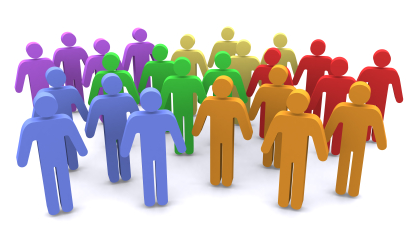
\includegraphics[width=1\textwidth]{graphics/knn-groups}
\par\end{center}
\begin{dinglist}{52}
\item \textcolor{magenta}{Utilization}: 

\begin{itemize}
\item we have a pile of objects that have been classified or labelled in
some way or other 
\item we have similar objects that have not yet been classified or labelled
\item we want to classify automatically the latter
\end{itemize}
\item Question: is \textcolor{magenta}{linear regression} applicable here?
Answer: it depends...

\begin{itemize}
\item LR requires an output that is a \textcolor{magenta}{continuous} variable---so,
NO
\item we can transform the categories into values using \textcolor{magenta}{thresholds}---so,
YES
\end{itemize}
\end{dinglist}

\foilhead{Mathematical Formulation of k-NN}

For 
\begin{itemize}
\item a given \textcolor{magenta}{value} of $k,$ 
\item and a prediction \textcolor{magenta}{point} $x_{0},$ 
\end{itemize}
the k-NN regression/classification is:
\begin{itemize}
\item \textcolor{magenta}{identify} first the $k$ training observations
that are the closest to $x_{0}$ in a neighborhood $\mathcal{N}_{0}$
\begin{itemize}
\item then \textcolor{magenta}{estimate} $y_{0}=f(x_{0})$ using the average
of all the responses in $\mathcal{N}_{0}$ in the case of a regression
\[
\hat{y}_{0}=\hat{f}(x_{0})=\frac{1}{k}\sum_{x_{i}\in\mathcal{N}_{0}}y_{i}
\]
\item or the \textcolor{magenta}{majority vote} in the case of a classification
(categories)---compute the conditional probability of a class $j$
as the proportion of points in $\mathcal{N}_{0}$ with response equal
to $j,$ 
\[
\Pr\left(Y=j\vert X=x_{0}\right)=\frac{1}{K}\sum_{i\in\mathcal{N}_{0}}I(y_{i}=j)
\]
 and classify the test observation, $x_{0}$ in the class with the
highest probability.
\end{itemize}
\end{itemize}

\foilhead{The k-NN procedure}
\begin{enumerate}
\item Choose a\textcolor{magenta}{{} distance/similarity metric}.
\item \textcolor{magenta}{Divide the labeled dataset} into \textcolor{magenta}{training
}and \textcolor{magenta}{test} data (usually 80-20).
\item Choose an\textcolor{magenta}{{} evaluation metric} (eg. the proportion
of misclassifications in the test set).
\item \textcolor{magenta}{Execute k-NN} several times, varying the value
of $k$ and checking the evaluation metric.
\item \textcolor{magenta}{Optimize $k$ }by choosing the value that yields
the best metric.
\item Create a \textcolor{magenta}{new test set} with the objects to classify
and repeat.
\end{enumerate}

\foilhead{Distance metrics}
\begin{description}
\item [{Euclidean~Distance}] for real-valued data
\item [{Cosine~Similarity}] between two real-valued vectors, $a$ and
$b$
\[
\cos\left(a,b\right)=\frac{a\cdot b}{\left\Vert a\right\Vert \left\Vert b\right\Vert },
\]
 which produces a value between $-1$ (opposite) and $1$(exactly
the same) with $0$ between the two, implying independence.
\item [{Jaccard~Distance}] between two sets of objects
\[
J(A,B)=\frac{\left|A\cap B\right|}{\left|A\cup B\right|},
\]
\item [{Hamming~Distance}] between 2 character strings or 2 words, (eg.
2 DNA sequences) where we loop over the each position and check whether
the letters are the same, if not we increment a counter by one. For
example, the distance between <<olive>> et <<ocean>> is $4,$
and that between ATCGA et CTGAA is $3.$ 
\item [{Mahlanobis~Distance}] take into account the correlation between
2 real-valued vectors
\[
d(a,b)=\sqrt{(a-b)^{T}S^{-1}(a-b)}
\]
and is invariant with respect to scale, where $S$ is the covariance
matrix
\item [{Manhattan}] distance between 2 real-valued vectors
\[
d(a,b)=\sum_{i=1}^{n}\left|a_{i}-b_{i}\right|
\]
\end{description}
\begin{rem*}
The choice of metric depends on the type of data... and must be made
based on experience.
\end{rem*}

\foilhead{Advantages et Disadvantages}
\begin{itemize}
\item Advantages:
\begin{dinglist}{52}
\item simple and efficient
\item no hypothesis on the underlying distribution of data (non-parametric)
\item rapid training phase
\end{dinglist}
\item Disadvantages:
\begin{dinglist}{56}
\item no model produced (a ``lazy'' method)
\item ``curse of dimensionality'' requiring a lot of memory when there
is a large number of features
\item need to treat outliers and missing values
\end{dinglist}
\end{itemize}

\foilhead{Training and Test Sets}
\begin{dinglist}{52}
\item 2 phases of all machine learning algorithms:

\begin{dinglist}{52}
\item a \textcolor{magenta}{training} phase where the model is created and
``learns'' how to treat the data
\item a \textcolor{magenta}{test }phase where we use new data to check how
good the model really is
\end{dinglist}
\end{dinglist}
\begin{example*}
Take a database with classification of individuals according to their
capacity to reimburse their credit (confidence rating) . The training
phase for k-NN consists simply of reading the data with points marked
``high'' or ``low'' and then classifying them as a function of
income. Then, for testing, we pretend not to know the rating and we
check the capacity of the algorithm to ``guess'' the good one. For
this, we extract 20\% of the data, drawn randomly from the database.
\end{example*}

\foilhead[-0.5in]{Example of k-NN - credit ratings}
\begin{lyxcode}
{\small >~head(data)}{\small\par}

{\small ~~~age~income~credit~}{\small\par}

{\small 1~~69~~~~3~~~~low~}{\small\par}

{\small 2~~66~~~57~~~~low~}{\small\par}

{\small 3~~49~~~79~~~~low~}{\small\par}

{\small 4~~49~~~17~~~~low~}{\small\par}

{\small 5~~58~~~26~~~~high}{\small\par}

{\small 6~~44~~~71~~~~high~}{\small\par}

{\small n.points~<-~1000~}{\small\textcolor{blue}{\#~number~of~lines~in~the~~dataset}}{\small ~}{\small\par}

{\small sampling.rate~<-~0.8~}{\small\par}

{\small\textcolor{blue}{\#~we~need~the~number~of~points~in~the~test~set~}}{\small\par}

{\small\textcolor{blue}{\#~to~compute~the~misclassification~rate}}{\small\par}

{\small num.test.set.labels~<-~n.points~{*}~(1~-~sampling.rate)~}{\small\par}

{\small\textcolor{blue}{\#~random~sample~of~lines~for~training~set}}{\small\par}

{\small training~<-~sample(1:n.points,~sampling.rate~{*}~n.points,~}{\small\par}

{\small ~~~~~~~~~~~~~~~replace=FALSE)~}{\small\par}

{\small train~<-~subset(data{[}training,~{]},~select~=~c(Age,~Income))~}{\small\par}

{\small\textcolor{blue}{\#~define~the~training~set~with~these~lines}}{\small\par}

{\small\textcolor{blue}{\#~the~other~lines~go~to~the~test~set}}{\small\par}

{\small testing~<-~setdiff(1:n.points,~training)~}{\small\par}

{\small\textcolor{blue}{\#~define~the~test~set~to~be~these~other~lines}}{\small\par}

{\small test~<-~subset(data{[}testing,~{]},~select~=~c(Age,~Income))~}{\small\par}

{\small cl~<-~data\$Credit{[}training{]}~}{\small\par}

{\small\textcolor{blue}{\#~subset~of~classes~for~training~set}}{\small\par}

{\small true.labels~<-~data\$Credit{[}testing{]}~}{\small\par}

{\small\textcolor{blue}{\#~subset~of~classes~for~test~set,~}}{\small\par}

{\small\textcolor{blue}{\#~we~retain~these...}}{\small\par}
\end{lyxcode}

\foilhead{Choice of evaluation metric }

How do we know/evaluate whether the model has done a good job? This
is often complicated and context-dependent, and a domain expert should
be consulted, if possible. 
\begin{dinglist}{56}
\item minimize false negatives---eg. in cancer diagnosis
\item compromise between \textcolor{red}{sensitivity} and \textcolor{red}{specificit}y

\begin{dinglist}{56}
\item sensitivity = the probability to \textcolor{magenta}{correctly diagnose}
a sick person as sick (rate of \textcolor{magenta}{true positives})
\item specificity = the probability to \textcolor{magenta}{correctly diagnose}
a healthy person as healthy (rate of \textcolor{magenta}{true negatives})
\end{dinglist}
\end{dinglist}
\begin{defn}
The \textcolor{red}{accuracy} is the ratio of the number of correct
labels and the total number of labels, and the \textcolor{red}{classification
error} is equal to one minus the accuracy.
\end{defn}

\foilhead{Putting it all together...}
\begin{dinglist}{52}
\item We now have:

\begin{itemize}
\item a measure of distance
\item an evaluation metric
\end{itemize}
\item For each individual in the test set:

\begin{itemize}
\item pretend not to know its label
\item look at the labels of the $k$ closest neighbors
\item use the label of the majority vote to label it
\item label in this way, all the members of the test set 
\item compute the classification error to measure our success
\end{itemize}
\end{dinglist}
\begin{itemize}
\item All of this is performed automatically in \textcolor{blue}{R }by a
single line:

\begin{itemize}
\item \texttt{\textcolor{blue}{knn (train, test, cl, k=3)}}
\end{itemize}
\item And, in \textcolor{blue}{scikit-learn}, by 2 lines
\begin{itemize}
\item \textcolor{blue}{knn = sklearn.neighbors.KNeighborsClassifier(n\_neighbors=3)}
\item \textcolor{blue}{knn.fit(X\_train, X\_test)}
\end{itemize}
\end{itemize}

\foilhead{The function \texttt{\textcolor{blue}{knn()}}}
\begin{itemize}
\item \texttt{\textcolor{blue}{knn()}} is part of the library \texttt{\textcolor{blue}{class}}
\item the function requires 4 inputs:

\begin{itemize}
\item (1) a matrix that contains the predictors associated to the training
set, \texttt{\textcolor{blue}{train.X}} 
\item (2) a matrix that contains the predictors associated to the data for
which we want to perform predictions, \texttt{\textcolor{blue}{test.X}} 
\item (3) a vector that contains the class for the training observations 
\item (4) a value of \texttt{\textcolor{blue}{k}}, the number of closest
neighbors, to be used by the classification algorithm
\end{itemize}
\end{itemize}

\foilhead[-0.5in]{The choice of k ?}

We try different values, in a given range, and observe how the evaluation
changes...
\begin{lyxcode}
{\small\textcolor{blue}{\#~loop~and~compute~~misclassification~rate}}{\small\par}

{\small\textcolor{blue}{\#~for~different~values~of~k~}}{\small\par}

{\small for~(k~in~1:20)~}{\small\par}

{\small\{}{\small\par}

{\small ~print(k)~}{\small\par}

{\small ~predicted.labels~<-~knn(train,~test,~cl,~k)~}{\small\par}

{\small ~}{\small\textcolor{blue}{\#~use~the~function~knn()}}{\small ~}{\small\par}

{\small ~num.incorrect.labels~<-~sum(predicted.labels~!=~true.labels)~~~}{\small\par}

{\small ~misclassification.rate~<-~num.incorrect.labels~/~}{\small\par}

{\small ~~~~~~~~~~~~~~~~~~~~~~~~~~~num.test.set.labels}{\small\par}

{\small ~print(misclassification.rate)~}{\small\par}

{\small\}}{\small\par}
\end{lyxcode}
Here is the program's output:
\begin{lyxcode}
{\small k~misclassification.rate~}{\small\par}

{\small 1,~0.28~}{\small\par}

{\small 2,~0.315~}{\small\par}

{\small 3,~0.26~}{\small\par}

{\small 4,~0.255~}{\small\par}

{\small 5,~0.23~}{\small\par}

{\small 6,~0.26~}{\small\par}

{\small 7,~0.25~}{\small\par}

{\small 8,~0.25~}{\small\par}

{\small 9,~0.235~}{\small\par}

{\small 10,~0.24}{\small\par}
\end{lyxcode}
We choose $k=5,$ which gives the lowest rate, and we apply it to
the classification of an individual age 57 with a revenue of 37 000:
\begin{lyxcode}
>~test~<-~c(57,37)~

>~knn(train,test,cl,~k~=~5)

{[}1{]}~low
\end{lyxcode}
\begin{rem*}
We used the function \texttt{\textcolor{blue}{knn()}} twice, with
a different objective each time. 
\end{rem*}
\begin{enumerate}
\item In the first call, the test set is a bunch of data used to evaluate
the model.
\item In the second, the ``test'' set is in fact a new data point for
which we seek a prediction. The algorithm does not distinguish whether
it is a real test, or whether we are predicting... 
\end{enumerate}

\foilhead{Modeling hypotheses by k-NN}
\begin{itemize}
\item The k-NN algorithm is an example of a \textcolor{magenta}{non parametric}
approach---there are no modeling hypotheses on the underlying probability
distributions.
\item But, there are other hypotheses:

\begin{itemize}
\item the notion of distance is valid in the space of data
\item the training data are classified into at least two categories
\item we choose the number of neighbors to use
\item we suppose that the observed features and the labels are related
\end{itemize}
\end{itemize}

\foilhead{References}
\begin{enumerate}
\item M. DeGroot, M. Schervish, \emph{Probability and Statistics}, Addison
Wesley, 2002.
\item Spiegel, Murray and Larry Stephens,\emph{ Schaum's Outline of Statistics,}
6th edition, McGraw Hill. 2017.
\item G. James, D. Witten, T. Hastie, R. Tibshirani. \emph{An Introduction
to Statistical Learning with Applications in R.} Springer. 2013.
\item Rachel Schutt and Cathy O\textquoteright Neil. \emph{Doing Data Science.}
O'Reilly. 2014.
\end{enumerate}

\end{document}
